  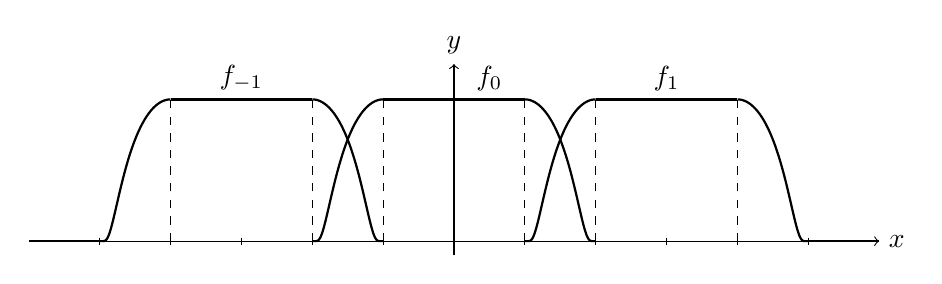
\begin{tikzpicture}[scale=0.9]

  % Eixos
  \draw[->] (-6,0) -- (6,0) node[right] {$x$};
  \draw[->] (0,-0.2) -- (0,2.5) node[above] {$y$};

  % f_{-1}
  \draw[
    domain=-4.999:-4.001,
    samples=120,
    smooth,
    thick
  ]
  plot (\x,{2*exp(1)*exp(-1/(1-(\x+4)^2))});

  \draw[thick] (-4,2) -- (-2,2);

  \draw[
    domain=-1.999:-1.001,
    samples=120,
    smooth,
    thick
  ]
  plot (\x,{2*exp(1)*exp(-1/(1-(\x+2)^2))});

  % f_0
  \draw[
    domain=-1.999:-1.001,
    samples=120,
    smooth,
    thick
  ]
  plot (\x,{2*exp(1)*exp(-1/(1-(\x+1)^2))});

  \draw[thick] (-1,2) -- (1,2);

  \draw[
    domain=1.001:1.999,
    samples=120,
    smooth,
    thick
  ]
  plot (\x,{2*exp(1)*exp(-1/(1-(\x-1)^2))});

  % f_1
  \draw[
    domain=1.001:1.999,
    samples=120,
    smooth,
    thick
  ]
  plot (\x,{2*exp(1)*exp(-1/(1-(\x-2)^2))});

  \draw[thick] (2,2) -- (4,2);

  \draw[
    domain=4.001:4.999,
    samples=120,
    smooth,
    thick
  ]
  plot (\x,{2*exp(1)*exp(-1/(1-(\x-4)^2))});

  % Parte zero
  \draw[thick] (-6,0) -- (-5,0);
  \draw[thick] (5,0) -- (6,0);

  % Linhas auxiliares
  \draw[dashed] (-4,0) -- (-4,2);
  \draw[dashed] (-2,0) -- (-2,2);

  \draw[dashed] (-1,0) -- (-1,2);
  \draw[dashed] (1,0) -- (1,2);

  \draw[dashed] (2,0) -- (2,2);
  \draw[dashed] (4,0) -- (4,2);

  % Labels
  \node at (-3,2.3) {$f_{-1}$};
  \node at (0.5,2.3) {$f_0$};
  \node at (3,2.3) {$f_1$};

  % Marcas
  \foreach \x in {-5,-4,-3,-2,-1,0,1,2,3,4,5}
    \draw (\x,0.05) -- (\x,-0.05);

\end{tikzpicture}

